\documentclass[../../../topic_calculus]{subfiles}

\begin{document}

\sectionline
\section{勾配ベクトルと臨界点}

山頂(極大)や谷底(極小)となる地点では、接平面は水平になっているはずである。

もし接している板が水平でなければ、その付近には必ず、より高い・低い方向があるため、そこは山頂や谷底とは呼べなくなる。

\br

ここで、\hyperref[thm:tangent-plane-equation]{接平面の方程式}は次のような形の式で表されていた。
\begin{review}
  $z=f(x,y)$上の点$(x_0,y_0,z_0)$における接平面の方程式は、
  \begin{equation*}
    z = \frac{\partial f}{\partial x}(x_0,y_0)(x - x_0) + \frac{\partial f}{\partial y}(x_0,y_0)(y - y_0) + z_0
  \end{equation*}
\end{review}

\br

$xyz$空間における水平な平面は、$z = z_0$($z_0$は定数)という形で表される。

\br

接平面の方程式が$z = z_0$という形になるためには、
\begin{equation*}
  \frac{\partial f}{\partial x}(x_0,y_0) = 0, \quad
  \frac{\partial f}{\partial y}(x_0,y_0) = 0
\end{equation*}
という条件が必要になる。

\br

この条件は、\hyperref[def:gradient]{勾配ベクトル}を使うとまとめて表すことができる。
\begin{equation*}
  \nabla f(x_0,y_0) = \vb*{o}
\end{equation*}
ここで、$\nabla f(x_0,y_0)$は、$\nabla f(x,y)$に$x = x_0,\, y = y_0$を代入したものである。

\begin{theorem}{勾配ベクトルと極値の関係}
  点$(x_0,y_0)$で$f(x,y)$が極大または極小ならば、
  \begin{equation*}
    \nabla f(x_0,y_0) = \vb*{o}
  \end{equation*}
\end{theorem}

このように、勾配ベクトルが零ベクトルとなる点$(x_0,y_0)$を、関数$f(x,y)$の\keywordJE{臨界点}{critical point}あるいは\keywordJE{停留点}{stationary point}という。

\subsection{臨界点と鞍点}

ただし、先ほど述べた定理の逆は成り立たない。

つまり、臨界点(勾配ベクトルが零ベクトル)だからといって、必ずしもその点で極大・極小になるとは限らないのである。
\begin{emphabox}
  \begin{spacebox}
    \begin{center}
      臨界点で極大・極小になるとは限らない
    \end{center}
  \end{spacebox}
\end{emphabox}

\br

たとえば、$z = x^2 - y^2$のグラフを考えてみよう。

\br

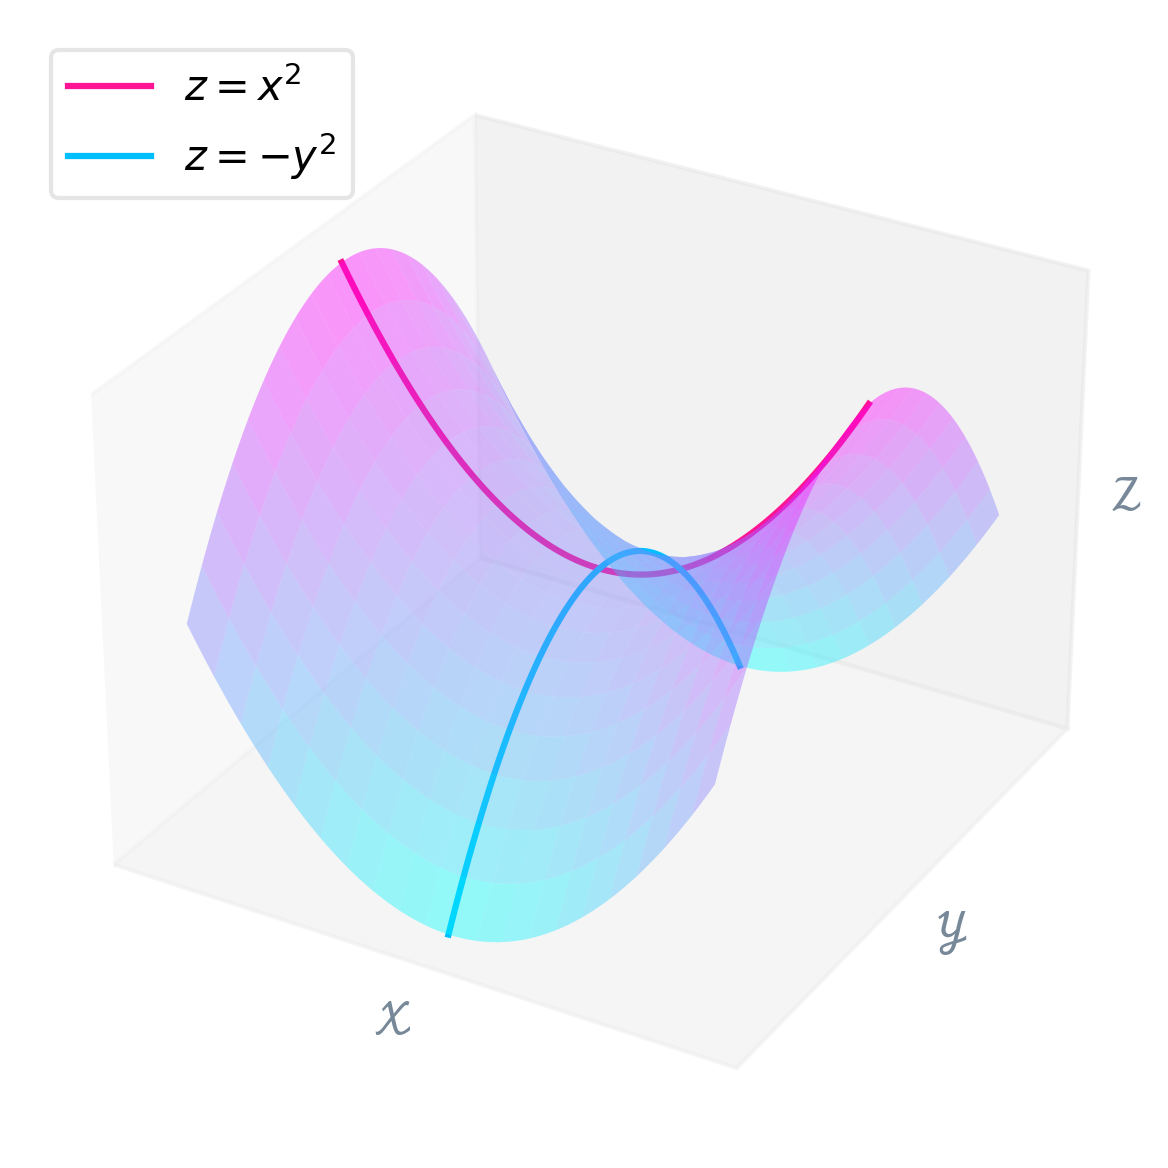
\includegraphics{../python/graph_x-pow2-sub-y-pow2_02.png}

勾配ベクトルを計算すると、
\begin{equation*}
  \nabla f(x,y) = \begin{pmatrix} 2x \\ -2y \end{pmatrix}
\end{equation*}
であるので、点$(0,0)$ではこの勾配ベクトルは零ベクトルとなる。

すなわち、点$(x,y) = (0,0)$は臨界点である。

\br

しかし、
\begin{itemize}
  \item $y=0$の場合のグラフ$z = x^2$は、$x=0$で極小
  \item $x=0$の場合のグラフ$z = -y^2$は、$y=0$で極大
\end{itemize}
となるので、$f(x,y) = x^2 - y^2$のグラフは、$(x,y) = (0,0)$で極大にも極小にもならない。

\end{document}
